\section{Problemstellung und Überblick}

%Softwaretests sind ein wichtiger Baustein f�r die Qualit�tssicherung von modernen Softwareprojekten.
%F�r Tests werden Testdaten spezifiziert. Auf deren Basis wird das Verhalten der Software gepr�ft.
%Bei Datenbank-basierten Anwendungen werden Testdaten in der Regel sehr umfangreich und komplex.
%
%Die Komplexit�t ergibt sich aus der Beschreibung von Beziehungen zwischen den einzelnen
%Datens�tzen. Besonders bei Systemen mit komplexen Datenbank-Schemata kann ein
%Testdaten-Modell schnell un�bersichtlich werden.
%
%F�r den Tester sind un�bersichtliche Testdaten aus verschiedenen Gr�nden ein Problem.
%Einerseits machen sie die Pflege fehleranf�llig. Andererseits ist es schwer,
%die modellierten Daten zu erfassen und zu verstehen. Tester w�nschen deshalb h�ufig Daten,
%die f�r mehrere Tests nutzbar sind. Dadurch reicht es aus, nur ein oder zumindest
%wenige Daten-Modelle zu verstehen und zu pflegen.
%
%Die im Rahmen einer Master Thesis [Quelle] entwickelte Modellierungssprache f�r Testdaten erlaubt
%eine �bersichtliche Modellierung von Testdaten. Sie ist einfach zu nutzen und integriert sich
%in g�ngige Entwicklungsumgebungen.
%
%Dar�ber hinaus wurde ein Algorithmus f�r die Generierung von Testdaten konzipiert. Das Ziel des
%Generators ist es, mit wenigen Datens�tzen viele Grenzf�lle bei Beziehungen abzudecken.



%
%\textbf{Aus FORUM Artikel}
%
%Zum Testen von Software-Anwendung, die Daten persistent in einem Datenbanksystem verwalten, werden Testdaten für die Datenbank benötigt. Für Anwendungen mit einem komplexen Datenbankschema ist die Spezifikation dieser Testdaten meist nicht trivial, da neben den Entitäten auch deren Beziehungen betrachtet werden müssen. Diese Beziehungen unterliegen in der Regel einer Menge komplexer fachlicher Regeln, die sich aus dem Domänen-Modell der Anwendung ergeben. 
%
%In dieser Arbeit wird untersucht, wie die zum Test von Datenbank-basierten Anwendungen notwendigen Testdaten auf einfache Weise beschrieben und automatisch erzeugt werden können.
%
%%---
%
%Eine zu prüfende Anwendung wird im Kontext von Software-Tests als System under Test (SUT) bezeichnet. Alle Voraussetzungen für einen Test werden dabei als sog. Test Fixture bezeichnet. Idealerweise soll die in einem Test Fixture beinhaltete Datenmenge für einen funktionalen Test eine hohe Testabdeckung bieten, dabei aber so klein und übersichtlich wie möglich sein. Somit sind die Testdaten einfacher zu verstehen und für eine große Anzahl von funktionalen Tests zu verwenden.
%
%Ein üblicher Ansatz, ein SUT in Verbindung mit einer Datenbank zu testen, ist das Testmuster Back Door Manipulation \cite{XUNIT_TEST_PATTERNS}. Idee hierbei ist, dass das Einspielen des Test Fixture in die Datenbank direkt durch den Test am SUT vorbei, d.h. sozusagen durch eine Hintertür, geschieht. Im ersten Schritt, dem Setup, wird die Datenbank über direkten Zugriff an dem SUT vorbei in den Anfangszustand des Test Fixture gebracht. Anschließend können im Exercise-Schritt die zu testenden Operationen am SUT durchgeführt werden. Die Überprüfung, ob sich das SUT richtig verhalten hat, findet im Verify-Schritt statt. Dabei kann der Zustand der Datenbank mit dem erwarteten Zustand des SUT verglichen, ebenfalls über die Test-eigene Datenbankverbindung. Abschließend können im vierten optionalen Schritt, Teardown, noch Aufräumarbeiten in der Datenbank implementiert sein.
%
%Basis für die nachfolgend beschriebenen Projektarbeiten ist die Java-Bibliothek Simple Test Utils for JUnit \& Co. (STU) zur Vereinfachung von Unit-Tests für Java-Anwendungen. STU steht unter der Apache License 2.0 und wird von der Firma Seitenbau entwickelt. Für Tests von Datenbank-basierten Anwendungen setzt STU auf der Bibliothek DbUnit [2] auf. DbUnit ist ein Framework zum Testen von Datenbank-basierten Java-Anwendungen. 
%
%Ziel des Projekts ist es u.a., funktionale Tests durch die Spezifikation eines Java-API und einer speziellen Testdatenbeschreibungssprache so zu vereinfachen, dass eine Datenbank einfach zu Beginn des Tests – über den Test selbst – in den wohldefinierten Anfangszustand das Test Fixture versetzt werden kann. Des Weiteren soll der erwartete Datenbank-Zustand am Testende einfach auf Basis des Test Fixture beschrieben werden können. Nach Ausführung des Tests soll automatisch der über das SUT erzeugte Datenbank-Zustand mit dem erwarteten Datenbank-Zustand verglichen und somit die Korrektheit der Anwendung geprüft werden können.

%%%----

%Alle Voraussetzungen für einen Test werden dabei als sog. Test Fixture bezeichnet. 
%%
%Idealerweise soll die in einem Test Fixture beinhaltete Datenmenge für einen funktionalen Test eine hohe Testabdeckung bieten, dabei aber so klein und übersichtlich wie möglich sein. Somit sind die Testdaten einfacher zu verstehen und für eine große Anzahl von funktionalen Tests zu verwenden.
%
%
%
%Ein üblicher Ansatz, ein SUT in Verbindung mit einer Datenbank zu testen, ist das Testmuster Back Door Manipulation \cite{XUNIT_TEST_PATTERNS}.
%
%Alle Voraussetzungen für einen Test werden dabei als \emph{Test Fixture} bezeichnet.
%%
%Ein üblicher Ansatz, ein SUT in Verbindung mit einer Datenbank zu testen, ist das Testmuster Back Door Manipulation \cite{XUNIT_TEST_PATTERNS}. Im Setup wird die Datenbank über direkten Zugriff an dem SUT vorbei in den Anfangszustand des Test Fixture gebracht. Anschließend können im Exercise-Schritt die zu testenden Operationen am SUT durchgeführt werden. Die Überprüfung, ob sich das SUT richtig verhalten hat, findet im Verify-Schritt statt. Dabei kann der Zustand der Datenbank mit dem erwarteten Zustand des SUT verglichen, ebenfalls über die Test-eigene Datenbankverbindung. 
%%Abschließend können im vierten optionalen Schritt, Teardown, noch Aufräumarbeiten in der Datenbank implementiert sein.

%%%%%---


Softwaretests sind ein wichtiger Baustein für die Qualitätssicherung von Softwareprojekten. Für Tests von Datenbank-basierten Anwendungen müssen u.a.~Testdaten für die Datenbank spezifiziert werden, auf deren Basis das Verhalten der zu testenden Software 
%(System Under Test, SUT) 
geprüft werden kann.
%
%
Die Spezifikation dieser Testdaten ist leider i.A.~sehr umfangreich und komplex und somit aufwändig und fehleranfällig.
%
%Bei datenbank-basierten Anwendungen sind die Testdaten meist sehr umfangreich und komplex.
%
Die Komplexität ergibt sich v.a.~aus der Beschreibung der Beziehungen zwischen den einzelnen Datensätzen.
%im Test Fixture.
%
Diese unterliegen einer Menge komplexer fachlicher Regeln, die sich aus dem Domänen-Modell und der Geschäftslogik der Anwendung ergeben.
%
Besonders bei Systemen mit großen oder komplexen Datenbank-Schemata kann ein Testdaten-Set schnell unübersichtlich werden.


Übergreifendes Ziel der hier beschriebenen Arbeit \cite{MT:Moll:2013} war es, die Spezifikation von Testdaten für Datenbank-basierte Java-Anwendungen zu vereinfachen.
%
Zum einen wurde hierzu eine geeignete Domänen-spezifische Sprache (DSL) für Testdaten entwickelt.
%
Die DSL erlaubt eine  übersichtliche Spezifikation von Testdaten, ist einfach zu nutzen und integriert sich in gängige Entwicklungsumgebungen.
%
Zum anderen wurde ein Generator zur automatischen Erzeugen von Testdaten implementiert. 
%
Das Ziel hierbei war es, mit möglichst wenig Datensätzen viele Grenzfälle bei Beziehungen abzudecken.
%
Basis der Entwicklungsarbeiten war die Java-Bibliothek Simple Test Utils for JUnit \& Co. (STU) zur Vereinfachung von Unit-Tests für Java-Anwendungen. STU steht unter der Apache License 2.0 und wird federführend von der Firma Seitenbau entwickelt. Für Tests von Datenbank-basierten Anwendungen setzt STU auf der Bibliothek DbUnit auf. 


\begin{figure}[tb]
	\begin{center}
		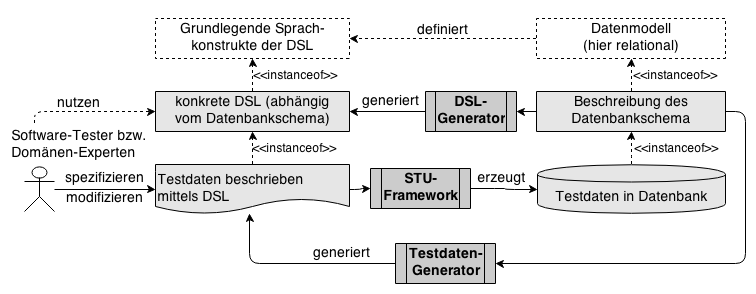
\includegraphics[width=12.5cm]{images/ansatz.png}
		\caption{\label{ansatz}Überblick über den gewählten Ansatz.}
	\end{center}
   %\vspace{-0.5cm}  %%% BAD HACK JW
\end{figure}

Abbildung \ref{ansatz} gibt einen Überblick über den im Projekt gewählten Ansatz.
%
Ausgangspunkt ist eine speziellen Beschreibung des relationalen Datenbankschemas (Details siehe \cite{MT:Moll:2013}).
%
Diese kann mittels eines Tools (nicht in der Abb.~dargestellt) manuell erstellt bzw. aus einer existierenden Datenbank extrahiert und ergänzt werden.
%
Aus der Beschreibung des Datenbankschemas wird die schema-abhängige Testdaten-DSL generiert. 
%
Diese DSL kann dann von den Software-Testern genutzt werden, um verschiedene Testdaten-Sets zu beschreiben und diese mittels STU in ihre Unit-Tests einzubinden.
%
Die mittels der DSL spezifizierten Testdaten werden dabei durch das STU-Frameworks automatisch in die Datenbank eingespielt (Backdoor-Manipulation \cite{XUNIT_TEST_PATTERNS}). 
%
Ausgehend von der Schema-Beschreibung können in der DSL beschriebene Test\-da\-ten-Sets automatisch generiert werden. Die generierten Testdaten können ggfls.~vor Verwendung noch modifiziert werden.
%
%
%
%Details und ausführliche Code-Beispiele zur Verwendung sind in \cite{MT:Moll:2013} zu finden.





	




